\documentclass[UTF8,12pt,a4paper]{ctexart}
\usepackage[top=2.1cm,bottom=2.1cm,left=2.25cm,right=2.25cm,headheight=17pt]{geometry}
\usepackage{amsmath,newtxmath,graphicx,booktabs,listings,tabularx,array}
\usepackage[table]{xcolor}
\usepackage{hyperref,fancyhdr,setspace,float,caption,lastpage,enumitem}
\setmainfont{Times New Roman}
\setsansfont{Arial}
\definecolor{Ink}{HTML}{213E50}
\definecolor{Muted}{HTML}{64717A}
\definecolor{Rule}{HTML}{CBD4DA}
\definecolor{Tint}{HTML}{EDF2F5}
\definecolor{CodeBG}{HTML}{F6F8F9}
\hypersetup{hidelinks,pdftitle={运动模糊点扩散函数的离散实现},pdfauthor={蔡斌}}
\setstretch{1.12}
\setlength{\parindent}{2em}
\setlength{\parskip}{2pt}
\setlength{\headheight}{17pt}
\AtBeginDocument{\setlength{\abovedisplayskip}{8pt}\setlength{\belowdisplayskip}{8pt}
\setlength{\abovedisplayshortskip}{4pt}\setlength{\belowdisplayshortskip}{6pt}}
\setlength{\intextsep}{10pt}
\setlength{\textfloatsep}{10pt}
\pagestyle{fancy}\fancyhf{}
\fancyhead[L]{\small\color{Muted}图像处理课程作业}
\fancyhead[R]{\small\color{Muted}运动模糊 PSF}
\fancyfoot[C]{\small\color{Muted}\thepage\,/\,\pageref*{LastPage}}
\renewcommand{\headrulewidth}{0.3pt}
\renewcommand{\headrule}{{\color{Rule}\hrule width\headwidth height\headrulewidth\vskip-\headrulewidth}}
\ctexset{section={format=\large\heiti\color{Ink},beforeskip=14pt,afterskip=9pt},
subsection={format=\normalsize\heiti\color{Ink},beforeskip=8pt,afterskip=5pt}}
\captionsetup{font=small,labelfont=bf,labelsep=quad,skip=6pt}
\captionsetup[table]{position=top}
\renewcommand{\arraystretch}{1.28}
\newcolumntype{Y}{>{\centering\arraybackslash}X}
\newcommand{\thead}[1]{\textbf{\color{Ink}#1}}
\renewcommand{\lstlistingname}{代码}
\lstdefinestyle{matlab}{language=Matlab,
basicstyle=\ttfamily\fontsize{9.6}{11.4}\selectfont,
keywordstyle=\bfseries\color{Ink},commentstyle=\color{Muted},
stringstyle=\color{Ink},numbers=left,
numberstyle=\ttfamily\fontsize{7.4}{8}\selectfont\color{Muted},numbersep=8pt,
frame=single,framerule=0.3pt,framesep=6pt,rulecolor=\color{Rule},
backgroundcolor=\color{CodeBG},breaklines=true,showstringspaces=false,
tabsize=4,columns=fullflexible,keepspaces=true,captionpos=t,literate={-}{{\char45}}1,
xleftmargin=1.4em,xrightmargin=0.5em,framexleftmargin=0.2em,
aboveskip=8pt,belowskip=9pt}
\begin{document}
\begin{center}
{\fontsize{22}{30}\selectfont\heiti\color{Ink}运动模糊点扩散函数的离散实现}\par\vspace{8pt}
{\small 蔡斌\qquad 数学jd2401\qquad 1024001338}\par\vspace{4pt}
{\small\color{Muted}2026 年 11 月 5 日}
\end{center}

\section{运动模型与离散构造}
由长度 \texttt{LEN} 和方向角 \texttt{THETA} 构造运动 PSF。
长度以像素计，角度从水平正方向逆时针起算\cite{doc}。
离散构造采用 MATLAB R2023b 的 \texttt{fspecial} 规则\cite{local}。

\subsection{连续运动模型}
设轨迹总长为 $L>0$，方向角为 $\theta$（弧度），运动中点位于原点。
均匀曝光下，连续核为
\begin{equation}
 h_c(x,y)=\frac{1}{L}\int_{-L/2}^{L/2}
 \delta(x-t\cos\theta)\,\delta(y-t\sin\theta)\,\mathrm dt.
\end{equation}
核的质量沿运动线段均匀分布，总积分为 1。

\subsection{半核网格}
离散构造取有效长度 $\ell$、离散线段半长 $a$ 和方向角 $\phi$：
\begin{equation}
 \ell=\max(1,\mathrm{LEN}),\qquad a=\frac{\ell-1}{2},\qquad
 \phi=\frac{\operatorname{mod}(\mathrm{THETA},180)}{180}\pi.
\end{equation}
例如，\texttt{LEN=9} 的水平核包含 9 个像素中心，首末中心间距为 8，故 $a=4$。
连续模型中的 $L/2$ 则表示轨迹半长。

记 $c=\cos\phi$、$s=\sin\phi$、$\sigma=\operatorname{sign}(c)$，
$\varepsilon=\texttt{eps}$。半核边界由方向确定：
\begin{equation}
 b_x=\operatorname{fix}(ac+\sigma-\ell\varepsilon),\qquad
 b_y=\operatorname{fix}(as+1-\ell\varepsilon).
\end{equation}
其中 \texttt{fix} 向零取整。网格坐标取 $x=0:\sigma:b_x$、$y=0:b_y$；
水平核和竖直核分别为行向量和列向量。

\subsection{端点权重与归一化}
有符号垂距为 $u=yc-xs$。
当 $\sqrt{x^2+y^2}\ge a$ 且 $|u|\le1$ 时，端点距离为
\begin{equation}
 d=\sqrt{u^2+\left(a-\left|\frac{x+us}{c}\right|\right)^2};
 \qquad\text{其余点取 }d=|u|.
\end{equation}
上式按双精度运算，竖直方向使用 \texttt{cos(pi/2)} 的计算值，约为
$6.123\times10^{-17}$。半核权重及镜像后的归一化分别为
\begin{equation}
 w=\max(1+\varepsilon-d,0),\qquad
 h=\frac{W}{\sum_{i,j}W_{ij}+\varepsilon\ell^2},
\end{equation}
其中 $W$ 为半核的镜像展开矩阵。输出按图像行坐标调整上下顺序。

\clearpage
\section{AI 初版与修改}
AI 初版以线段穿过像素方格的长度作为权重，完整函数见代码~\ref{code:initial}。
\lstinputlisting[style=matlab,caption={AI 初版的轨迹积分实现},label={code:initial}]{motion_psf_ai.m}
初版采用 $p(t)=p_0+td$、$0\le t\le1$，而 $d$ 是单位向量，
对应的轨迹长度为 1 像素。将裁剪参数的分母由 \texttt{d(k)} 改为
\texttt{p1(k)-p0(k)} 后，参数区间覆盖端点之间的整条线段。

\begin{table}[H]\centering\small
\caption{\texttt{LEN=9} 时的参数化修正结果}\label{tab:initial}
\begin{tabularx}{\linewidth}{YYYYr}
\toprule
\rowcolor{Tint}\thead{角度} & \thead{初版尺寸} & \thead{修正后尺寸} & \thead{内置尺寸} & \thead{修正后最大误差}\\
\midrule
$0^\circ$ & $1\times1$ & $1\times9$ & $1\times9$ & $2.637\times10^{-16}$\\
$45^\circ$ & $2\times2$ & $7\times7$ & $7\times7$ & $5.743\times10^{-2}$\\
$90^\circ$ & $1\times1$ & $9\times1$ & $9\times1$ & $2.637\times10^{-16}$\\
\bottomrule
\end{tabularx}
\end{table}

表~\ref{tab:initial} 中，参数化修正恢复了矩阵尺寸；$45^\circ$ 下的权重误差为 $0.05743$。
这一差异来自离散方式：初版按方格内轨迹长度积分，目标核按像素中心距离和端点位置赋权。
最终函数据此采用第 1 节的半核构造。


\clearpage
\section{函数实现}
函数依次完成半核取样、端点赋权、镜像展开和归一化。
输入为有限实数 \texttt{double} 标量，\texttt{LEN>0}；默认值为
\texttt{LEN=9}、\texttt{THETA=0}。
\lstinputlisting[style=matlab,caption={运动模糊 PSF 函数},label={code:final}]{motion_psf.m}

\clearpage
\section{测试结果}
在 MATLAB R2023b（23.2.0.2365128）中，以
\texttt{fspecial('motion',LEN,THETA)} 为参照，比较输出尺寸及逐元素系数。
表~\ref{tab:checks} 的 1489 组参数和 2 种默认调用均通过 \texttt{isequal}。
\begin{table}[H]\centering
\caption{最终函数与内置函数的对照}\label{tab:checks}
\begin{tabularx}{\linewidth}{lXrr}
\toprule
\rowcolor{Tint}\thead{测试组} & \thead{参数覆盖} & \thead{一致数量} & \thead{最大误差}\\
\midrule
常规参数 & 8 个长度 $\times$ 13 个角度 & 104/104 & 0\\
边界参数 & 11 个长度 $\times$ 35 个角度 & 385/385 & 0\\
随机参数 & 均匀抽取长度与角度 & 1000/1000 & 0\\
默认调用 & 无参数、仅指定长度 & 2/2 & 0\\
\bottomrule
\end{tabularx}
\end{table}
\noindent\small 最大误差定义为 $\max_{i,j}|h_{ij}-h^{\mathrm{ref}}_{ij}|$。\normalsize

\begin{figure}[H]\centering
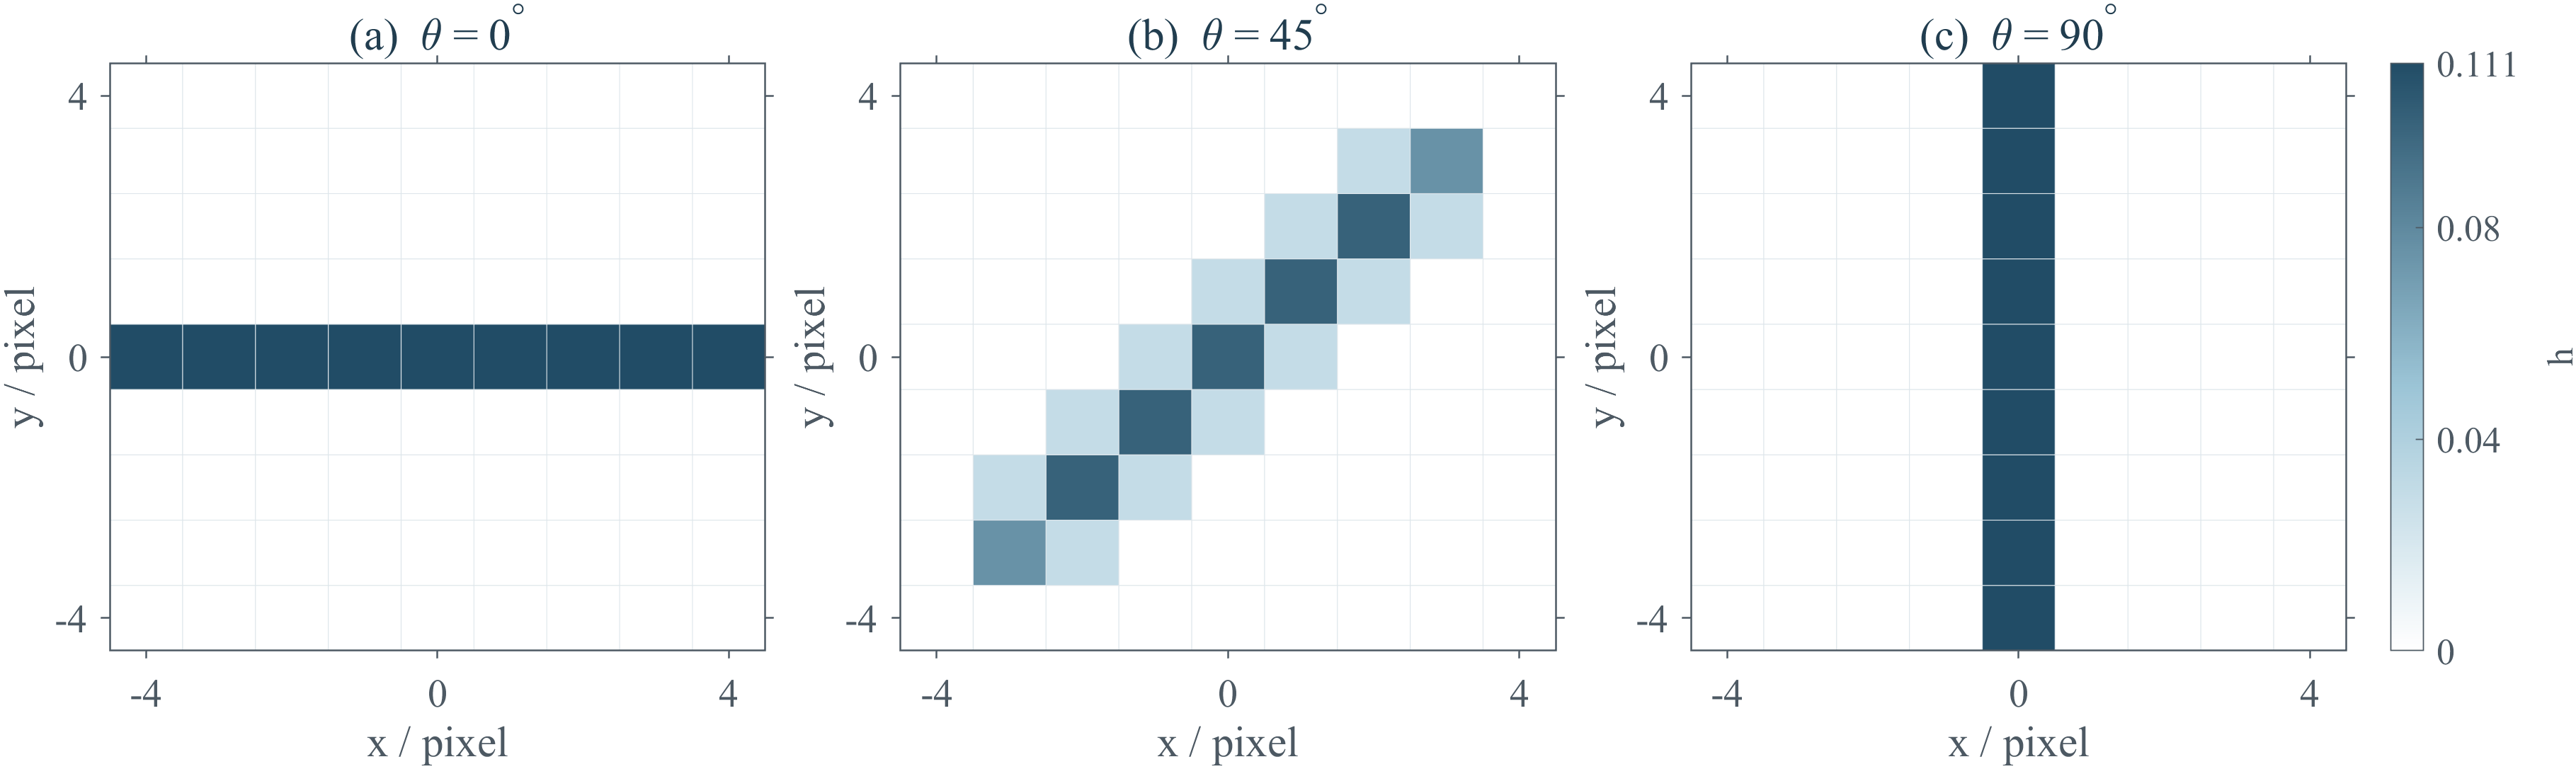
\includegraphics[width=\linewidth]{截图/psf_kernels.png}
\caption{\texttt{LEN=9} 的方向核，原始尺寸依次为 $1\times9$、$7\times7$ 和 $9\times1$。}
\label{fig:kernels}
\end{figure}
图~\ref{fig:kernels} 采用直角坐标，各核居中补零至 $9\times9$ 并共用色标。
边界与随机测试的 1385 个输出均为有限非负系数，满足中心对称；
系数和与 1 的最大偏差为 $2.243\times10^{-14}$。

\subsection*{测试参数}
\begingroup
\noindent\textbf{\color{Ink}常规组合}\par
\noindent 长度：$[0.25,1,1.25,2.5,5,9,13.7,20]$。\par
\noindent 角度：
$[-180,\allowbreak-90,\allowbreak-45,\allowbreak0,\allowbreak30,\allowbreak45,\allowbreak89.5,\allowbreak90,\allowbreak135,\allowbreak180,\allowbreak225,\allowbreak270,\allowbreak360]^\circ$。
\par\vspace{3pt}\noindent\textbf{\color{Ink}边界与随机组合}\par
\noindent 边界长度覆盖 $\varepsilon$、1 与 9 的邻域及 100；角度覆盖
$-180^\circ$ 至 $360^\circ$ 间各 $90^\circ$ 倍数及左右邻域。
\par\noindent 随机长度取自 $[0.05,100.05)$，角度取自 $[-720,720)$；
使用 \texttt{twister}，种子为 20261105。
\par\endgroup

\clearpage
\section{AI 交互记录}
图~\ref{fig:ai1}--\ref{fig:ai3} 按问答原文摘录排版，展示代码生成、差异分析与结果核验。
\setlength{\intextsep}{5pt}
\begin{figure}[H]\centering
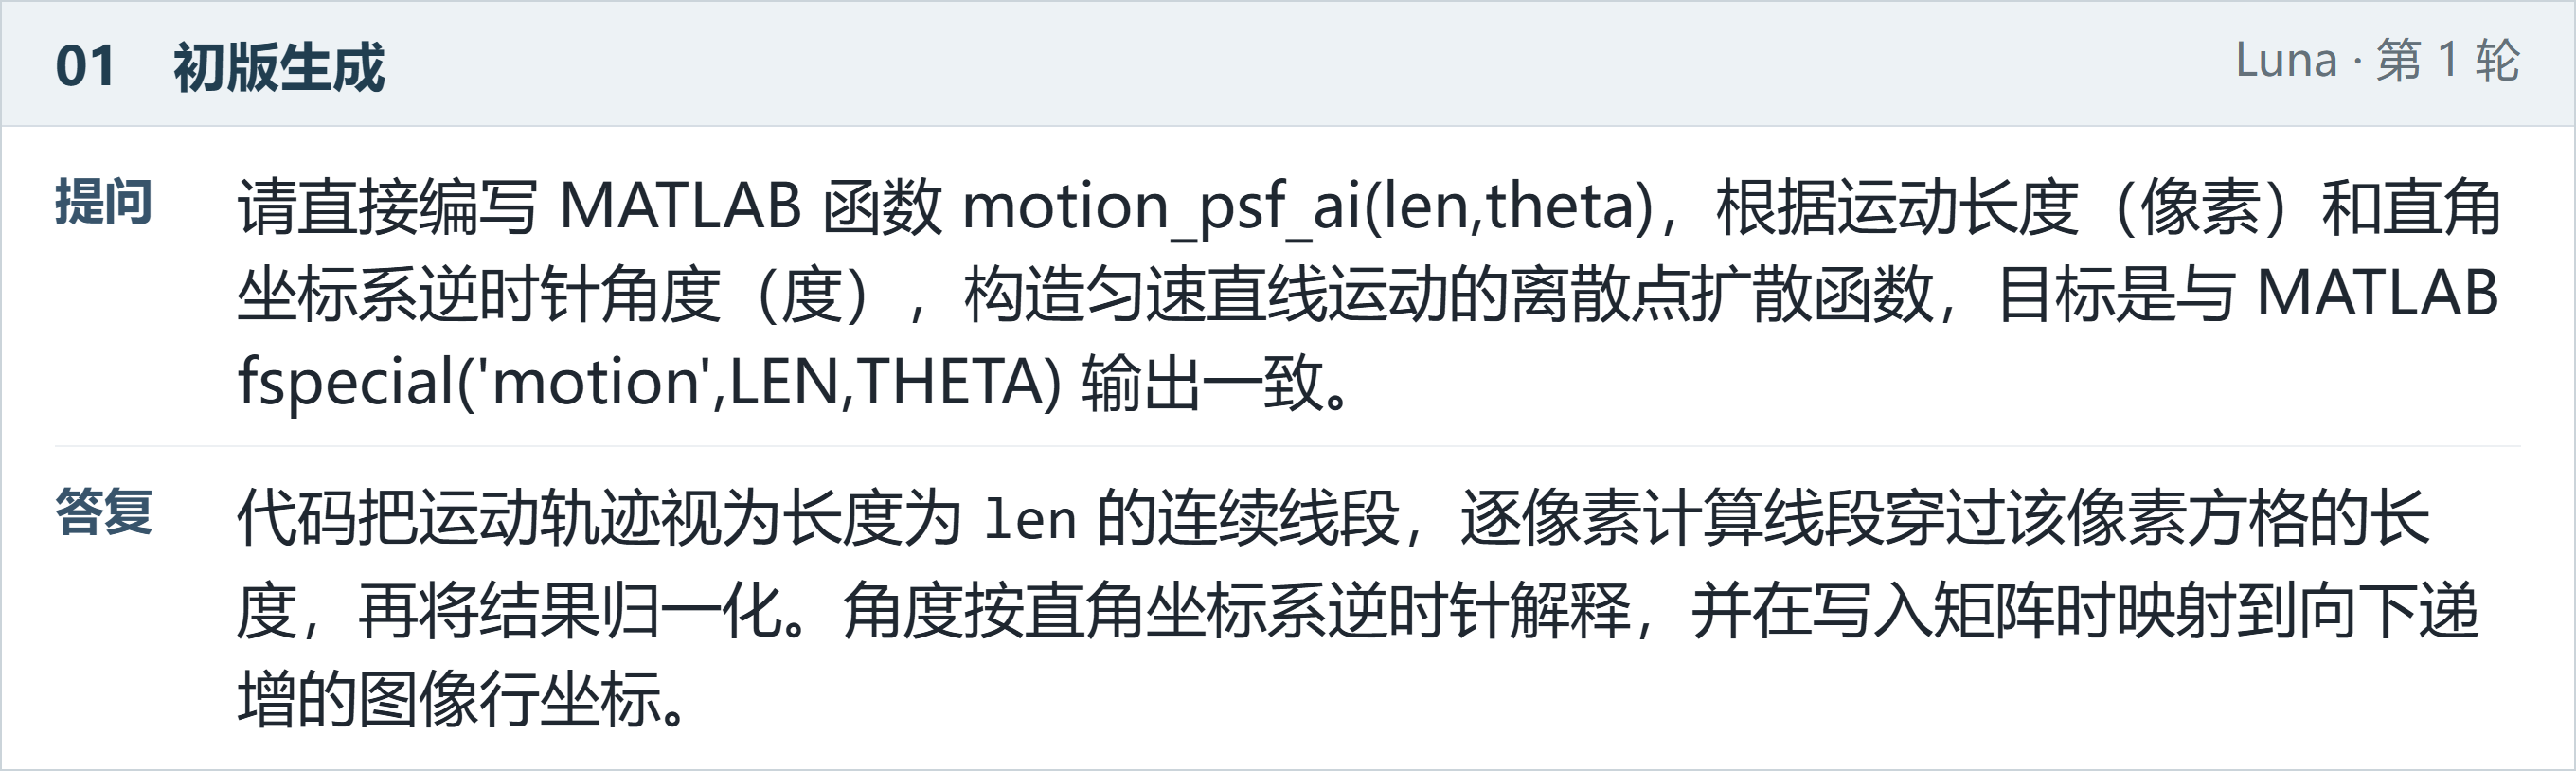
\includegraphics[width=\linewidth]{交互记录/01_初版生成.png}
\caption{初版函数的生成}\label{fig:ai1}
\end{figure}
\begin{figure}[H]\centering

\includegraphics[width=\linewidth]{交互记录/02_差异分析.png}
\caption{参数化修正与离散权重分析}\label{fig:ai2}
\end{figure}
\begin{figure}[H]\centering

\includegraphics[width=\linewidth]{交互记录/03_最终核验.png}
\caption{最终函数与输出核验}\label{fig:ai3}
\end{figure}
\begingroup\small\raggedright
\renewcommand{\refname}{参考资料}
\begin{thebibliography}{9}
\setlength{\itemsep}{0pt}\setlength{\parskip}{0pt}
\bibitem{doc} MathWorks. \emph{fspecial: Create predefined 2-D filter}.
\url{https://www.mathworks.com/help/images/ref/fspecial.html}.
\bibitem{local} MathWorks. MATLAB R2023b，\texttt{fspecial.m}，
\texttt{motion} 分支，第 190--225 行。
\end{thebibliography}
\endgroup
\end{document}
